\documentclass{article}

% Language setting
% Replace `english' with e.g. `spanish' to change the document language
\usepackage[english]{babel}

% Set page size and margins
% Replace `letterpaper' with `a4paper' for UK/EU standard size
\usepackage[letterpaper,top=2cm,bottom=2cm,left=3cm,right=3cm,marginparwidth=1.75cm]{geometry}

\usepackage{amsmath}
\usepackage{color}
\usepackage{listings}
\usepackage{algorithm}
\usepackage{algpseudocode}
\usepackage[utf8]{inputenc}
\usepackage{graphicx} %LaTeX package to import graphics
\graphicspath{{images/}} %configuring the graphicx package
\usepackage[export]{adjustbox}
\usepackage{subcaption}
\newcommand\numberthis{\addtocounter{equation}{1}\tag{\theequation}}
\DeclareMathOperator{\sign}{sign}

% Define code listing style
\lstdefinestyle{mystyle}{
    backgroundcolor=\color{backcolour},   
    commentstyle=\color{codegreen},
    keywordstyle=\color{magenta},
    numberstyle=\tiny\color{codegray},
    stringstyle=\color{codepurple},
    basicstyle=\ttfamily\footnotesize,
    breakatwhitespace=false,         
    breaklines=true,                 
    captionpos=b,                    
    keepspaces=true,                 
    numbers=left,                    
    numbersep=5pt,                  
    showspaces=false,                
    showstringspaces=false,
    showtabs=false,                  
    tabsize=2
}

% Set code listing style
\lstset{style=mystyle}

\geometry{a4paper, margin=1in}
\usepackage[colorlinks=true, allcolors=black]{hyperref}
\begin{document}

\title{rSVD and related Applications}
\author{Cenzato, Pisante, Procaccio}
\date{\today}
\maketitle
\begin{figure}[h]
    \centering
    \includegraphics[width=0.4\linewidth]{20151029123608!Logo_Politecnico_Milano.png}
\end{figure}
\newpage


\tableofcontents
\newpage

\section*{Introduction}

This project delves into a comprehensive investigation at the convergence of Image Compression, Principal Component Analysis (PCA), Singular Value Decomposition (SVD), and QR Decomposition, utilizing the capabilities of the C++ programming language. This undertaking surpasses mere theoretical abstraction, involving the practical implementation of algorithms and the introduction of specialized data structures to amplify computational efficiency.

This report begins with the description of the Image Compression Algorithm elucidating the theoretical foundations. The subsequent Testing and Results section systematically explores and substantiates claims with empirical evidence.

Moving into the domain of Principal Component Analysis (PCA), an introductory discourse lays the groundwork, explaining PCA's role in dimensionality reduction. A meticulous Overview of PCA Algorithm follows, delving into the intricacies of the method, culminating in a presentation of practical insights derived from systematic Test Results.

The academic trajectory extends to Singular Value Decomposition (SVD), where the robustness of the algorithm is demonstrated through the incorporation of the Power Method. A nuanced exploration of rSVD, the role of the Gaussian Matrix in SVD, and an analytical scrutiny of obtained Results collectively underscore the computational efficiency achieved. This section concludes with an examination of the Moore-Pensrose Pseudoinverse within the SVD framework.

The exploration persists with an examination of QR Decomposition, commencing with a formal Overview of Givens Algorithm. This section includes a detailed exploration of parallelization strategies using OpenMP and MPI, complemented by methodical General Observations and Recommendations. Additionally, the discourse extends to the Householder Algorithm, elucidating parallelization strategies and expounding on pivotal Computational Considerations.

The academic discourse concludes with an examination of the meticulously crafted Matrix Implementation, covering critical facets such as Transposition, Multiplication, and the strategic incorporation of Lazy Evaluation. Rigorous evaluation through systematic Benchmarks provides a quantitative lens into the computational efficiency of the custom matrix implementation.



\newpage
\setcounter{section}{0}
\section{Image Compression}
\subsection{Introduction}
To compress a matrix $A$, we seek an approximation requiring significantly less storage space. Randomized Singular Value Decomposition (rSVD) proves advantageous for this purpose. SVD decomposes $A$ into three matrices, $U$, $\Sigma$, and $V$, ordered by their contributions to $A$. This ordering facilitates efficient approximation by retaining only the most significant components of these matrices.

For compression, a parameter $k$ is chosen to determine the number of singular values considered for the approximation. A higher $k$ improves approximation quality but also increases the data required for encoding. The compression process involves selecting only the first $k$ columns of matrices $U$ and $V$, and the upper-left $(k \times k)$ square of $\Sigma$, which contains the $k$ largest (and therefore most important) singular values. Additionally, the oversampling factor $p$ can be added to retrieve addiditional information. 

Images can be represented through three color channels: red, green, and blue, each as a $(m \times n)$ matrix with values ranging from 0 to 255. Alternatively, images can be in grayscale, where each pixel is represented by a single intensity value. In the context of compression, we will focus on compressing the matrices representing individual color channels.

It's worth noting that a similar approach can be employed for grayscale images, where the compression is achieved through the decomposition of a single intensity matrix. This versatility allows for an efficient compression strategy that adapts to both color and grayscale representations.


\subsection{Overview of Image Compression algorithm}
The C++ code utilizes Singular Value Decomposition (SVD) for image compression, setting parameters for rank $r$ and oversampling $p$. It loads a PNG image using the STB library, instantiates the `APPLICATIONS` class, and measures compression time. The code adapts to RGB or grayscale, applying rSVD-based compression accordingly. After compression, a backward conversion restores the image. Key metrics like uncompressed size, compressed size, ratio, and duration are computed. The decompressed image is saved, and memory is freed. The pseudocode succinctly outlines these steps in the \texttt{main} function.
\begin{algorithm}
\caption{Main Function for Image Compression}
\begin{algorithmic}[1]
\Procedure{main}{}
    \State Set compression parameters $r$ and $p$
    \State Set input and output file paths
    \State Load input image from file
    \If{RGB image}
        \For{each color channel}
            \State Perform image compression using rSVD
            \State Perform backward conversion to obtain decompressed image
        \EndFor
    \Else
        \State Perform image compression using rSVD (grayscale)
        \For{each color channel}
            \State Perform backward conversion to obtain decompressed image
        \EndFor
    \EndIf
    \State Save decompressed image to file
    \State Free allocated memory
    \State \textbf{return} 0
\EndProcedure
\end{algorithmic}
\end{algorithm}
In addition, such algorithm has been parallelized with openmp. In particular, the compression of the 3 colours is done in parallel. This provides a good speedup of the process.

\subsection{Testing and results}
The compression testing was conducted on an input image Figure~\ref{fig:Original_image} in PNG format. The image underwent processing in both RGB and grayscale formats, yielding substantial results.
\begin{figure}[h]
    \centering
    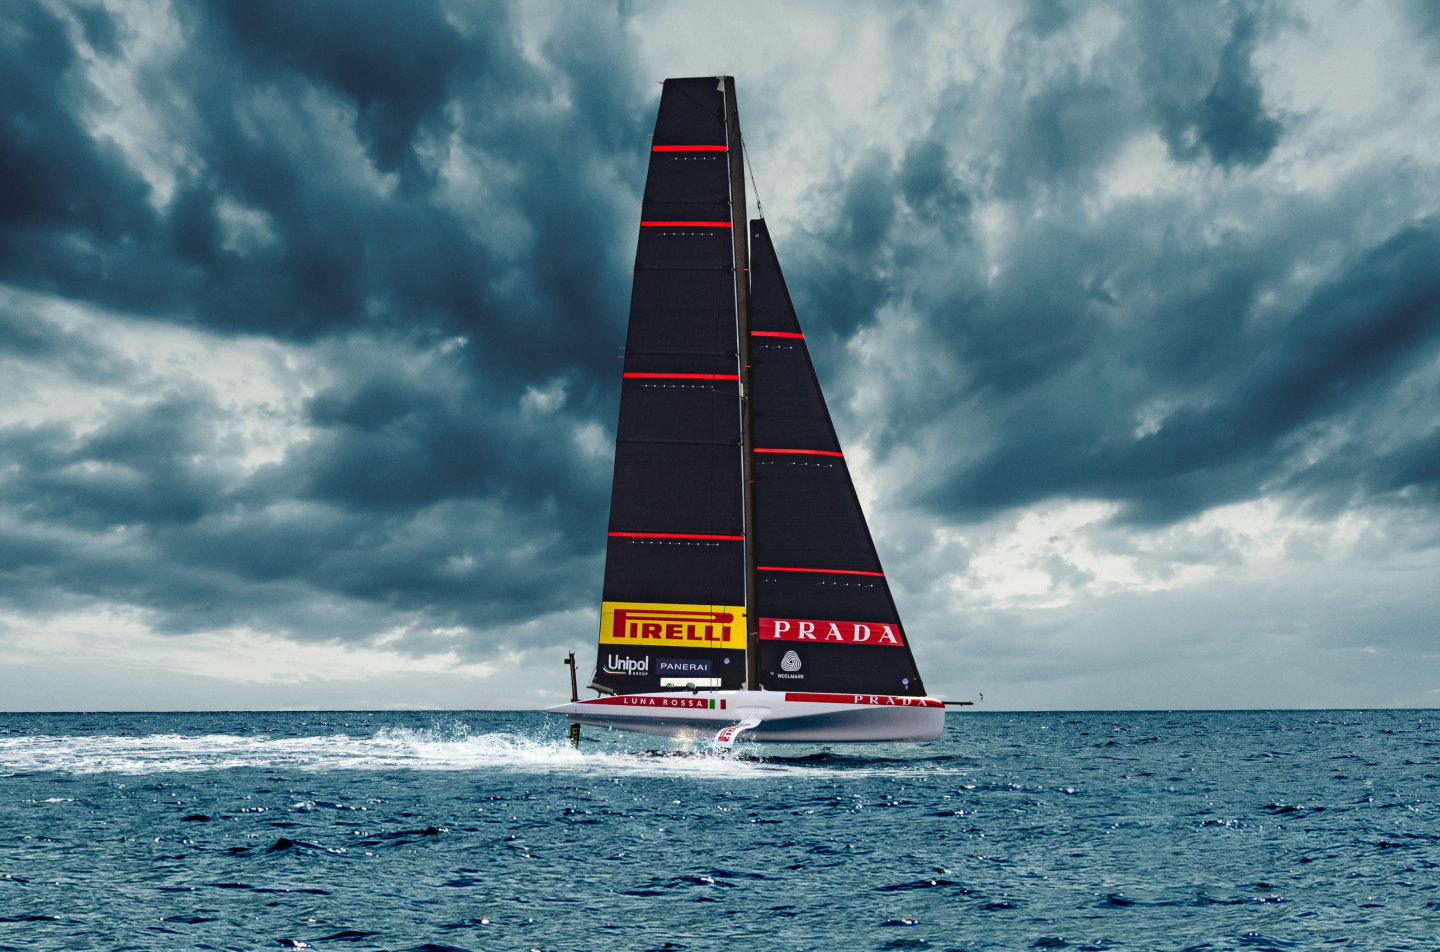
\includegraphics[width=0.4\linewidth]{luna_rossa.png}
    \caption{Original image}
    \label{fig:Original_image}
\end{figure}
In particular, the results are depicted in Figure~\ref{fig:group_of_four}. It is evident that the choice of the target rank has substantial implications. For a smaller value of \(r\), the compressed image exhibits a good approximation of the input image, placing a specific emphasis on key features such as the boat and sail shape, text on the boat, and the horizon. Additionally, the brightness of colors is well-preserved.

\begin{figure}
    \centering

    \subfloat[r=100, p=10]{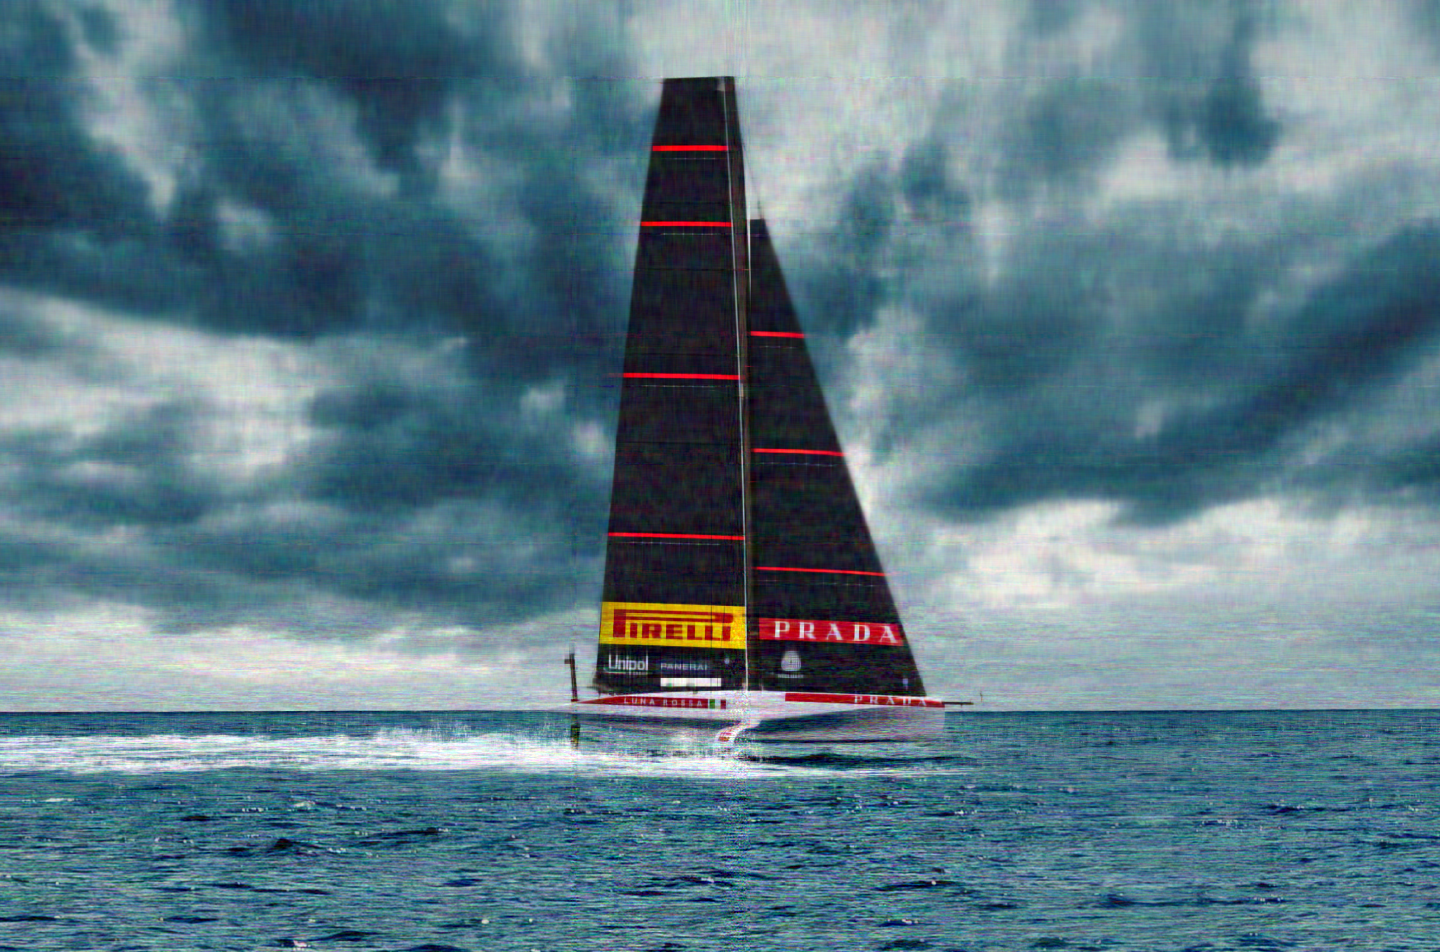
\includegraphics[width=0.35\textwidth]{luna_rossa_out10010}\label{fig:lr100}}
    \hfill
    \subfloat[r=50, p=10]{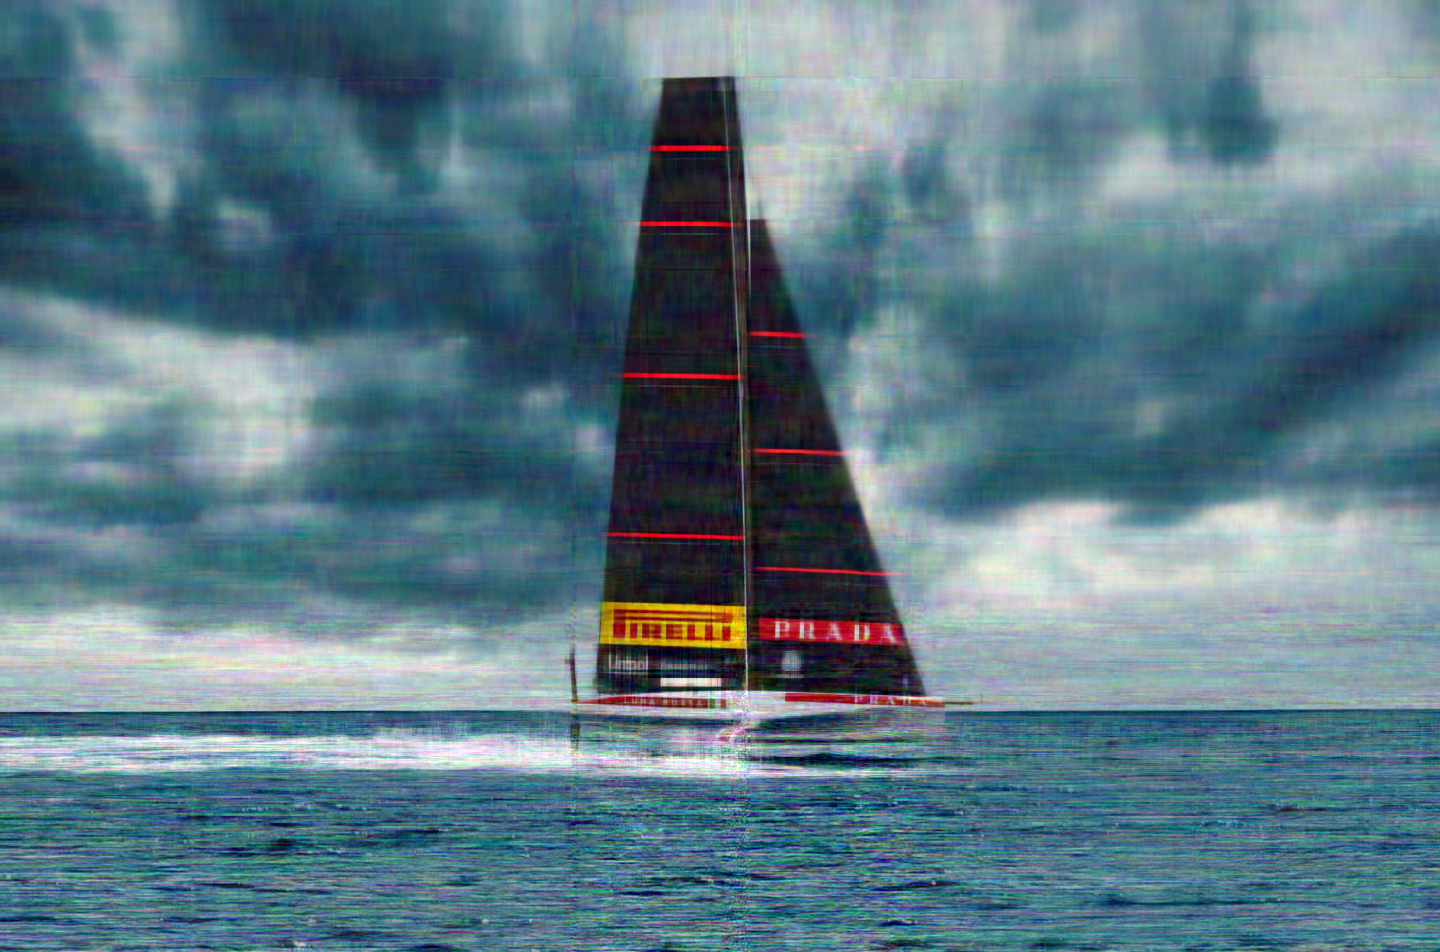
\includegraphics[width=0.35\textwidth]{luna_rossa_out5010.png}\label{fig:lr50}}

    \vspace{1em} % Spacing between the rows of images

    \subfloat[r=12, p=10]{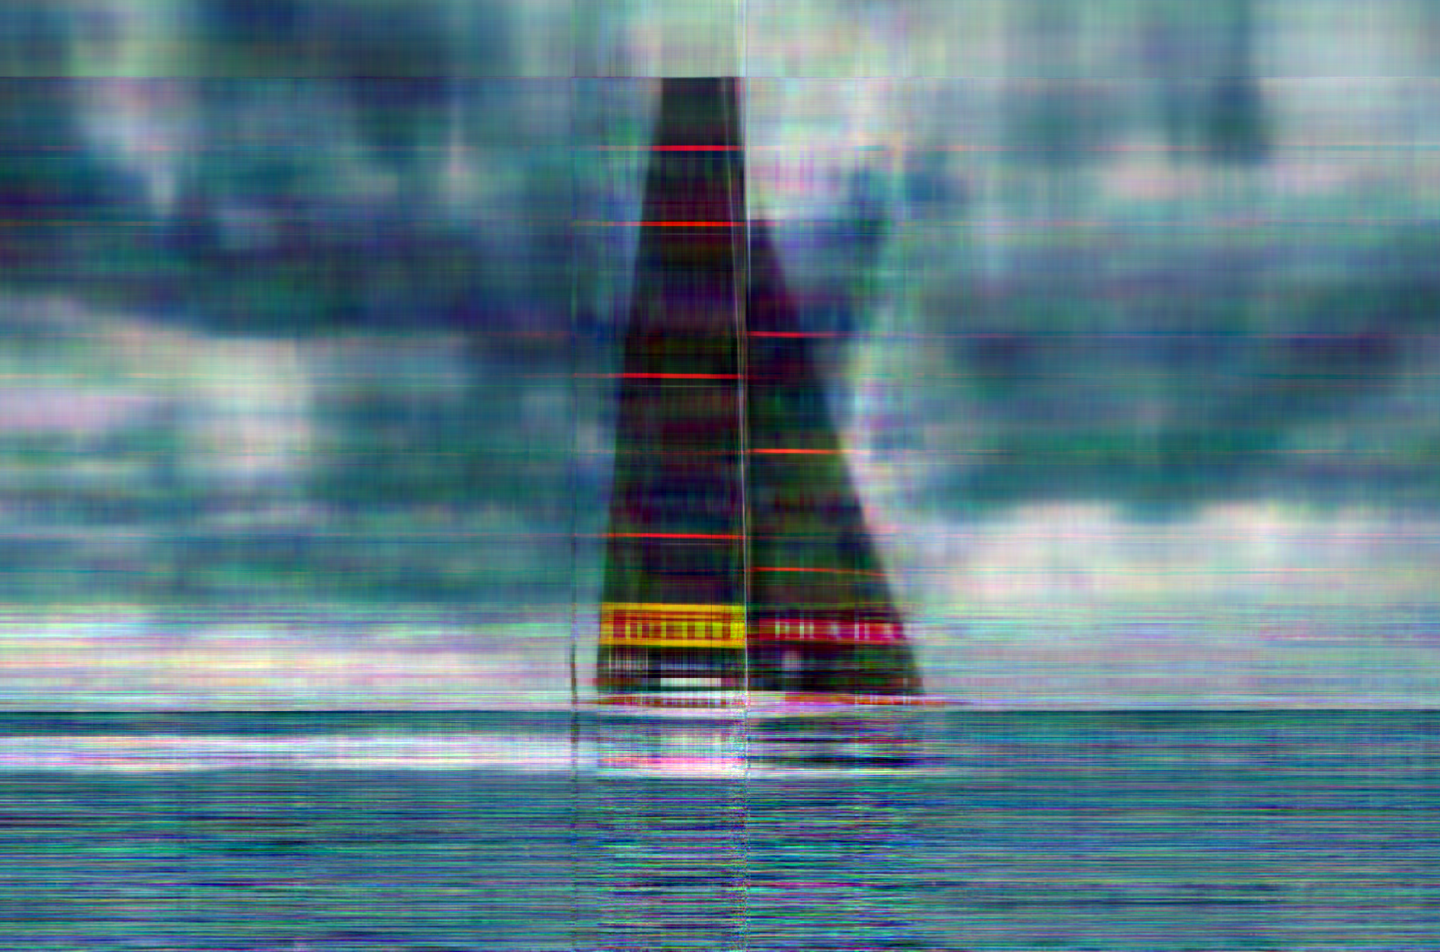
\includegraphics[width=0.35\textwidth]{luna_rossa_out1210.png}\label{fig:lr12}}
    \hfill
    \subfloat[r=2, p=10]{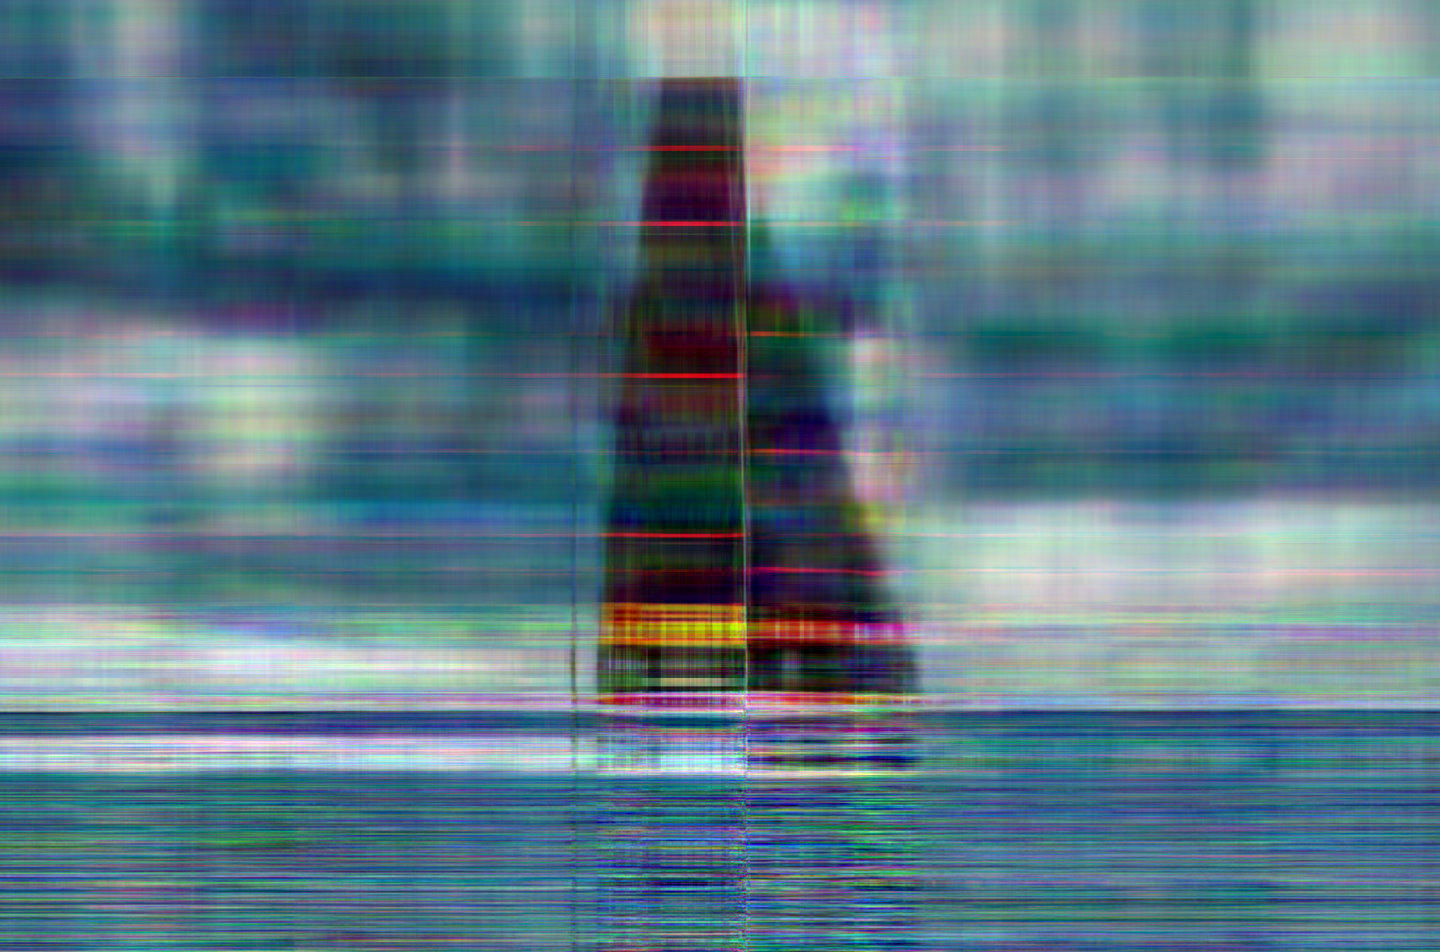
\includegraphics[width=0.35\textwidth]{luna_rossa_out0210.png}}\label{fig:lr02}

    \caption{Results for different target ranks}
    \label{fig:group_of_four}
\end{figure}


In addition the Figure~\ref{fig:variance} shows the cumulative variance with respect to the target rank. It's worth noticing that the first 20 components detain around 80\% of the total information.
\begin{figure}[h]
    \centering
    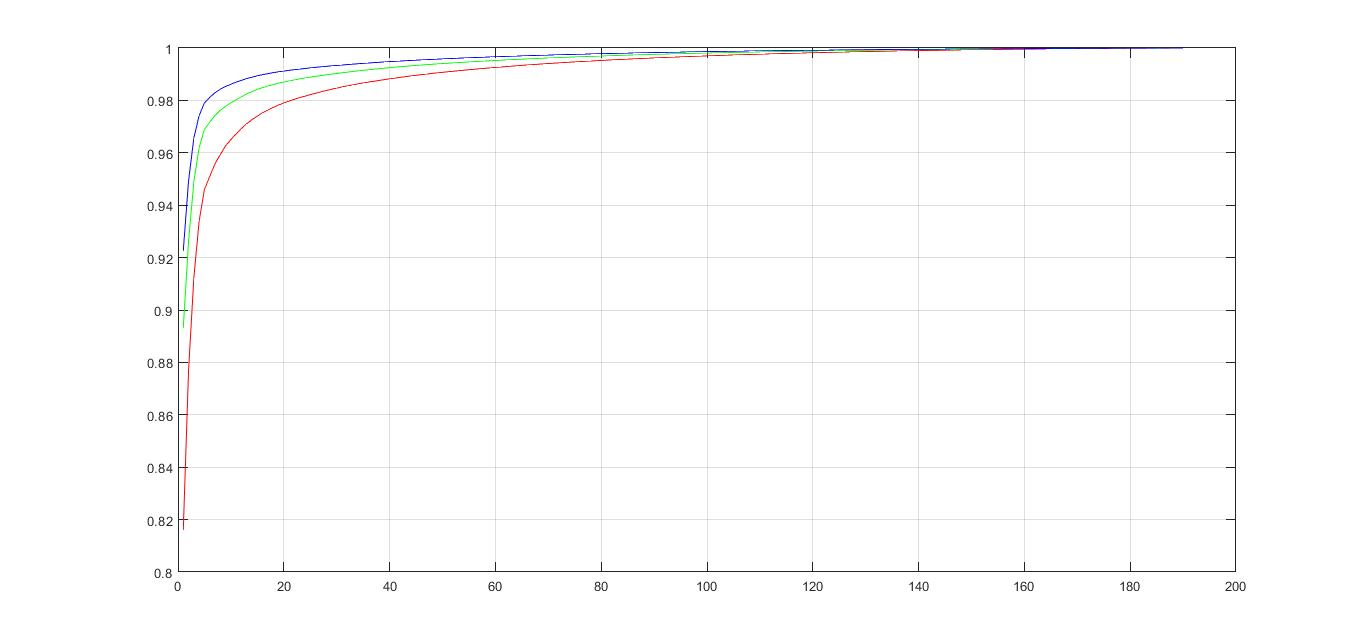
\includegraphics[width=0.4\linewidth]{imagecomprvar.jpg}
    \caption{Cumulative variance}
    \label{fig:variance}
\end{figure}

It is essential to highlight that the algorithm has also been implemented for grayscaling. Specifically, grayscale values can be obtained by applying one of three available grayscaling methods within the dedicated function:
\vspace{\baselineskip}

\[
\text{{grayscaleImage}}(i, j) = \frac{{0.21 \cdot \text{{red}} + 0.72 \cdot \text{{green}} + 0.07 \cdot \text{{blue}}}}{{255.}}
\]

\[
\text{{grayscaleImage}}(i, j) = \frac{{\text{{red}} + \text{{green}} + \text{{blue}}}}{3 \cdot 255.}
\]

\[
\text{{grayscaleImage}}(i, j) = \frac{{\text{{max}}(\text{{red}}, \text{{green}}, \text{{blue}}) + \text{{min}}(\text{{red}}, \text{{green}}, \text{{blue}})}}{2 \cdot 255.}
\]

\newpage

\section{PCA}

\subsection{Introduction}
Principal Component Analysis (PCA) is a widely used technique in the field of multivariate analysis and statistics. It provides a powerful tool for extracting essential information from high-dimensional datasets by identifying and capturing the most significant patterns within the data.

PCA aims to transform the original variables of a dataset into a new set of uncorrelated variables called principal components. These components are ordered by their significance, with the first component explaining the most variance in the data. By selecting a subset of the top principal components, one can achieve dimensionality reduction while retaining the essential features of the dataset. In this test, we explore the application of PCA as a dimensionality reduction method and its role in uncovering the latent structures and relationships present in a given dataset.

\subsection{Overview of the PCA algorithm}
For the implementation of PCA we use a randomized Singular Value Decomposition (rSVD) approach. The rSVD algorithm leverages randomization techniques to efficiently approximate the principal components of a matrix, making it suitable for large-scale datasets. Additionally, we preprocess the data by centering it before applying the rSVD. 

\begin{algorithm}
\caption{Principal Component Analysis (PCA)}
\begin{algorithmic}[1]
\Function{pca}{$A, r$}
    
    \If{$m > n$}
        \State $X \gets A$
    \Else
        \State $X \gets A.\text{transpose()}$
    \EndIf

    \For{$i \gets 0$ \textbf{to} $m-1$}
        \State Compute mean for each row
        \State Subtract the mean over row to every element of the row
    \EndFor

    \State $(U, s, V) \gets \text{obj.rsvd}(X, r)$

    \If{$using A$}
            \State \textbf{return} $U \cdot s.\text{asDiagonal}()$
    \Else \Comment{If using $A^\top$}
        \State \textbf{return} $U.\text{transpose()} \cdot X$
    \EndIf
\EndFunction
\end{algorithmic}
\end{algorithm}


\subsection{Test results}
In particular, we performed the principal component analysis (PCA) on a dataset from the FDA-NCI Clinical Proteomics Program Databank.

Each column of the dataset represents measurements taken from a patient. There are 216 columns representing 216 patients, out of which 121 are ovarian cancer patients and 95 are normal patients.

Each row represents the ion intensity level at a specific mass-charge value indicated in MZ. There are 2000 mass-charge values, and each row represents the ion-intensity levels of the patients at that particular mass-charge value.

\vspace{\baselineskip}
\begin{figure}[h]
\centering
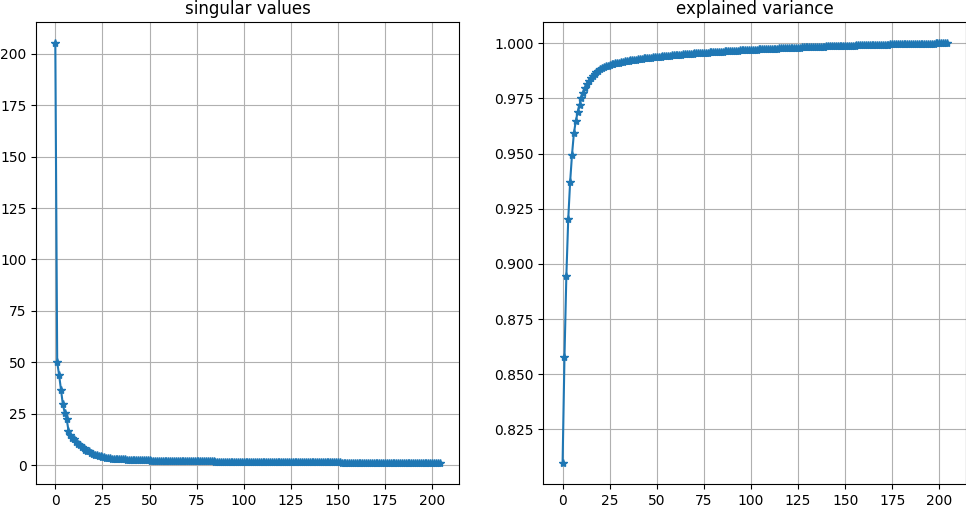
\includegraphics[width=0.55\linewidth]{pca_explained_variance200.png}
\caption{\label{fig:pca1}plot of the explained variance of the dataset.}
\end{figure}

\begin{figure}
    \centering

    \subfloat[r=100, p=10]{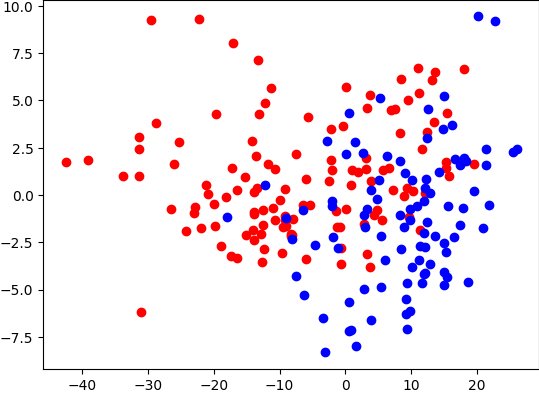
\includegraphics[width=0.4\textwidth]{pca_2scatterplot.png}\label{fig:sub1}}
    \hfill
    \subfloat[r=50, p=10]{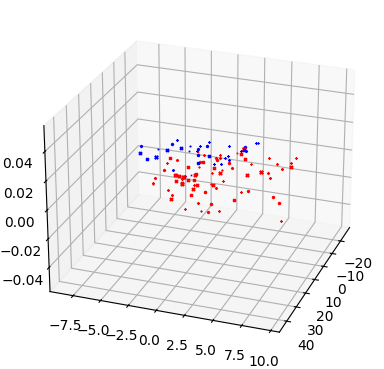
\includegraphics[width=0.4\textwidth]{pca_3scatterplot.png}\label{fig:sub2}}
\end{figure}

This dataset has an extensive array of features, making a comprehensive analysis challenging. To address this complexity, we applied Principal Component Analysis (PCA).

As illustrated in {figure} [h], the singular values exhibit a rapid decline. Moreover, we observe that the first three singular values explain nearly 90\% of the dataset's variance.


Observing the scatterplots presented in Figures~\ref{fig:pca2} and \ref{fig:pca3}, it becomes evident that a separation between patients with and without cancer is achieved by considering only the first two or three principal components. This highlights the effectiveness of dimensionality reduction through Principal Component Analysis (PCA) in elucidating patterns indicative of cancer presence in the dataset.



\newpage



\section{Singular Value Decomposition}
Having explored the principles and applications of Principal Component Analysis (PCA) and Image Compression, we now turn our attention to the underlying mathematical technique : Singular Value Decomposition (SVD). It is a matrix factorization technique that decomposes a given matrix into three separate matrices, revealing essential information about the structure and properties of the original matrix.

For a given matrix \( A \in \mathbb{R}^{m \times n} \), the SVD factorization is expressed as:

\begin{align}
    A & = U \Sigma V^T \\
\end{align}
where:
\begin{align}
    U & : \text{Left singular vectors matrix} \in \mathbb{R}^{m \times m} \\
    \Sigma & : \text{semi-Diagonal matrix of singular values} \in \mathbb{R}^{m \times n} \\
    V^T & : \text{Transpose of right singular vectors matrix} \in \mathbb{R}^{n \times n}
\end{align}

The diagonal elements of $\Sigma$ represent the singular values, and the columns of $U$ and $V$ are the left and right singular vectors, respectively. Notably, SVD is applicable to any matrix, regardless of its size or properties.


\subsection{SVD with Power Method}
The SVD can be computed using the Power Method. The latter is an algorithm which converges to the eigenvector that corresponds to the maximal eigenvalue of the matrix taken into consideration.

\vspace{\baselineskip}
    The pseudo-algorithm used to compute the SVD is the following:

\begin{algorithm}
\caption{SVD with Power Method}
\begin{algorithmic}[3]
\Function{SVDwithPM}{$A$}

    \While{$i < k$}
        \State $B \gets A^\top \cdot A$
        \State $v \gets \text{PowerMethod}(B)$
        \State $\sigma \gets \lVert A \cdot v \rVert$

        \If{$\sigma > \epsilon$}
            \State $u \gets A \cdot v \cdot (1 / \sigma)$
            \State $A \gets A - (\sigma \cdot u \cdot v^\top)$
            \State $i \gets i + 1$
        \EndIf
    \EndWhile

    \State \textbf{return} $(U, s, V)$
\EndFunction
\end{algorithmic}
\end{algorithm}

Being \( k = \min(m, n) \), where \( m \) and \( n \) are the dimensions of the matrix.

The iterations continue until one of the following conditions is met:

1. If the matrix is of full rank, iterate until reaching the minimum dimension of the matrix (\( k \)).

2. If the computed eigenvalue is almost equal to zero (up to a given tolerance), stop the iteration.

\vspace{\baselineskip}
As for the power method I first considered the following algorithm:
\begin{algorithm}
\caption{Power Method for Eigenvalue Estimation}
\begin{algorithmic}[1]
\Function{PowerMethod}{$A$}
    \State Initialize $v$ as a Gaussian vector with $\|v\| = 1$
    \State Compute $B \gets A^\top \cdot A$
    \State $err \gets \infty$
    
    \While{$err > \epsilon$}
        \State $v \gets B \cdot v$
        \State $v \gets \frac{v}{\|v\|}$
        \State $err \gets \|v_{\text{old}} - v\|$
    \EndWhile

    \State \textbf{return} $v$
\EndFunction
\end{algorithmic}
\end{algorithm}

Let \(v_i\) be the eigenvector computed at iteration \(i\) and \(v_{i-1}\) be the eigenvector computed at the previous iteration. The stopping criteria for the algorithm is defined as follows:

\[ \lVert v_i - v_{i-1} \rVert < \epsilon \]

where \(\lVert \cdot \rVert\) represents the norm of a vector, and \(\epsilon\) is a given tolerance value.

\vspace{\baselineskip}
However, this algorithm requires the computation of the matrix \(B = A^T \cdot A\), which can pose challenges since the computation of the multiplication is very expensive. To address these issue, an alternative algorithm is considered, focusing only on the matrices \(A\) and \(A^T\).

\begin{algorithm}
\caption{Power Method for Singular Value Decomposition}
\begin{algorithmic}[1]
\Function{PowerMethod}{$A$}
    \State Initialize $v$ as a Gaussian vector of size $A.\text{rows()}$ with $\|v\| = 1$

    \While{$err > \epsilon$}
        \State $v_{\text{old}} \gets v$
        \State $u \gets A \cdot v$
        \State $u \gets \frac{u}{\|u\|}$
        \State $v \gets A^\top \cdot u$
        \State $v \gets \frac{v}{\|v\|}$
        \State $err \gets \|v_{\text{old}} - v\|$
    \EndWhile

    \State \textbf{return} $(u, v)$
\EndFunction
\end{algorithmic}
\end{algorithm}



\subsection{rSVD}
   Another algorithm implemented in this class is the randomized SVD. This algorithm is particularly advantageous for analyzing large matrices as it reduces dimensionality. Given a matrix \(A\) of size \(m \times n\) and a target rank \(r\), the algorithm proceeds as follows:

\begin{algorithm}
\caption{Randomized SVD (rSVD) Algorithm}
\begin{algorithmic}[1]
\Function{rsvd}{$A, r, p, q$}
    \State $P \gets \text{generate a gaussian matrix of dimensions n x k}$ 
    
    \State $U \gets A \cdot P$ \Comment{$U$ is of size $m \times k$}

    \For{$i \gets 0$ \textbf{to} $q-1$}
        \State $U \gets A \cdot (A^\top \cdot U)$
    \EndFor

    \State $(Q, U) \gets \text{QR.Givens\_solve\_parallel}(U)$
    \State $\text{QR.setQR\_for\_svd\_parallel}(Q, U)$

    \State $Q \gets Q.\text{topLeftCorner}(m, k)$

    \State $Y \gets Q^\top \cdot A$ \Comment{$Y$ is of size $k \times n$}

    \State $(U_y, s, V) \gets \text{svd\_with\_PM}(Y)$
    \State $U \gets Q \cdot U_y$

    \State \textbf{return} $(U, s, V)$
\EndFunction
\end{algorithmic}
\end{algorithm}

   The resulting SVD is an approximation of the original matrix $A$, with only the first $r$ singular values and corresponding singular vectors computed.

\subsection{Gaussian matrix}
The \texttt{SVD::genmat} function generates a random matrix of dimensions $m \times n$ filled with values sampled from a standard normal distribution (with mean $0$ and standard deviation $1$). The function utilizes OpenMP for parallelization to enhance computational efficiency.

\begin{itemize}
    \item \textbf{Matrix Initialization:} The function initializes a matrix $M$ of size $m \times n$ to store the generated random values.
    
    \item \textbf{Parallelization with OpenMP:} The function utilizes OpenMP directives to parallelize the loop responsible for generating random values.
    
    \item \textbf{Thread-Specific Random Seeds:} Within the parallel section, each thread obtains a unique random seed by adding its thread rank to the value obtained from \texttt{std::random\_device}. This ensures that each thread generates distinct random values.
\end{itemize}

\subsubsection*{MPI Parallelized Matrix Generation}

The \texttt{genmat} function employs MPI parallelization to generate a random matrix distributed among different processes. It calculates the distribution of rows among processes, and generates local matrices on each process. Random values are sampled from a standard normal distribution, and the local matrices are gathered to construct the global matrix.


\subsubsection*{Comments}

An observation from our experiments reveals that the MPI version outperformed the OpenMP implementation when dealing with large matrix dimensions, such as $5000 \times 5000$. However, it is noteworthy that our typical application scenarios involve smaller matrices, typically on the order of $1 \times 10^{-3}$.

The parallelization choices were made to optimize the performance of the function in diverse computing environments. While the MPI version demonstrated superior efficiency with larger matrices, the OpenMP approach remains relevant for smaller matrices, balancing the trade-off between computational resources and scalability.


\subsection{Results}
Several tests were conducted to validate the efficiency and correctness of the proposed methods. The tolerance \(\epsilon\) was set to \(10^{-8}\), and the tests were performed on matrices of increasing size generated randomly within the range of -10 to 10.

\begin{enumerate}
\item $10 \times 10$ matrix

SVD with Power Method:

Time of execution power method 1-st algorithm: 0.00329849 s

\( \text{PM1} : \| A - U \Sigma V^T \| = 1.05767 \times 10^{-14} \)

Time of execution power method 2-nd algorithm: 0.004897 s

\( \text{PM2} : \| A - U \Sigma V^T \| = 1.11608 \times 10^{-14} \)

Difference eigenvalues = 8.98115e-15

\vspace{\baselineskip}
rSVD ( r = 5 ):

Time of execution rSVD algorithm: 0.00694928 s

\(\| A - U \Sigma V^T \| = 19.3972 \)

Speed Up randomized = 0.474652

Norm of difference first r eigenvalues = 0.235447

\vspace{\baselineskip}
\item $100 \times 100$ matrix

SVD with Power Method:

Time of execution power method 1-st algorithm: 3.36989 s

\( \text{PM1} : \| A - U \Sigma V^T \| = 3.00817 \times 10^{-13} \)

Time of execution power method 2-nd algorithm: 2.95494 s

\( \text{PM2} : \| A - U \Sigma V^T \| = 3.15329 \times 10^{-13} \)

Difference eigenvalues = 1.62896e-13

\vspace{\baselineskip}
rSVD ( r = 60 ):

Time of execution rSVD algorithm: 1.27542 s

\(\| A - U \Sigma V^T \| = 148.793 \)

Speed Up randomized: 2.64219

Norm of difference first r eigenvalues = 0.179286

\vspace{\baselineskip}
\item $1000 \times 200$ matrix

SVD with Power Method:

Time of execution power method 1-st algorithm: 65.0099 s

\( \text{PM1} : \| A - U \Sigma V^T \| = 1.86931 \times 10^{-12} \)

Time of execution power method 2-nd algorithm: 532.937 s

\( \text{PM2} : \| A - U \Sigma V^T \| = 2.00974 \times 10^{-12} \)

Difference eigenvalues = 1.53411e-12

\vspace{\baselineskip}
rSVD ( r = 160 ):

Time of execution rSVD algorithm: 43.7981 s

\(\| A - U \Sigma V^T \| = 908.887 \)

Speed Up randomized: 1.48431

Norm of difference first r eigenvalues = 0.436731
\end{enumerate}
\vspace{\baselineskip}

From these tests it can be seen that:
\begin{itemize}
\item In the algorithm using the Power Method, the error in the reconstruction of the matrix from the Singular Value Decomposition (SVD) is consistently low, approaching the machine epsilon, across all conducted tests. This suggests a highly accurate factorization. Additionally, the two distinct Power Methods produce nearly identical eigenvalues.

\item In the randomized SVD (rSVD) method, the error in the factorization is comparatively higher. However, this discrepancy is deemed acceptable, given the nature of rSVD as an approximation method. The primary objective of rSVD is to expedite computation, and the introduced error is considered reasonable in light of this objective. Indeed, a speedup is observed in comparison to the first algorithm utilizing the power method (the speedup is clearly dependent on the target rank used in the rSVD). Furthermore, the computed eigenvalues in the randomized approach demonstrate a high degree of similarity to those obtained through a non-randomized methodology.

\item In the third test, it becomes evident that the initial algorithm employed for the power method performs better when applied to non-square matrices. This is attributed to its capability to effectively reduce dimensionality in such scenarios.

\item Finally, the correctness of the algorithms has been tested by comparing the results obtained from the SVD with the ones obtained using python.

\end{itemize}

Additionally, from the depicted plot, it is evident that with an increment in target ranks, the error norm in the factorization of a 150 x 150 Gaussian random matrix, computed using the rSVD method, decreases. This observation aligns with expectations, as the execution time also proportionally increases.

\begin{figure}[h]
    \centering
    \includegraphics[width=0.55\linewidth]{rsvd.png}
    \caption{\label{pca1}rSVD with incrementing target rank.}
    \end{figure}


    \subsection{Moore-Pensrose pseudoinverse}
    The Moore-Penrose Pseudoinverse provides a generalization of the matrix inverse for non-square matrices or matrices that may not have a unique inverse (for example if they are not full rank).  
    
    Its computation uses the Singular Value Decomposition.
    
    \begin{algorithm}
    \caption{Calculate Pseudoinverse}
    \begin{algorithmic}[1]
    \Function{pseudoinverse}{$A$}
        \State \Comment{Perform Singular Value Decomposition on matrix $A$}
        \State $(U, s, V) \gets \text{svd\_with\_PM}(A)$
    
        \For{$i \gets 0$ \textbf{to} $k-1$} \Comment{Number of singular values}
            \State $s[i] \gets \frac{1}{s[i]}$  \Comment{Invert singular values}
        \EndFor
    
        \State{Multiply inverted singular values with the transposed matrices}
    \EndFunction
    \end{algorithmic}
    \end{algorithm}
    
    It's worth highlighting that with this algorithm, there is no need to verify whether the singular value is non-zero. This is because the Singular Value Decomposition (SVD) exclusively includes eigenvalues that are non-zero along with their associated eigenvectors.
\newpage

\section{QR Decomposition}

QR factorization is a fundamental numerical technique used in linear algebra to decompose a matrix into the product of an orthogonal matrix and an upper triangular matrix. This factorization plays a crucial role in various applications, including solving systems of linear equations, least squares problems, and eigenvalue computations.

The decomposition of a matrix $A$ into the product $A = QR$ involves obtaining an orthogonal matrix $Q$ and an upper triangular matrix $R$. The orthogonal matrix $Q$ captures the rotation and reflection components, while the upper triangular matrix $R$ contains the essential information about the original matrix.

In this report, we delve into the QR factorization process, specifically focusing on two distinct algorithms: the Givens rotation and the Householder reflection. These algorithms provide numerical methods to transform a given matrix into its QR factorization, each with its unique approach to introducing zeros below the main diagonal.

The Givens algorithm employs sequential rotations to eliminate elements below the diagonal, while the Householder algorithm uses successive reflections to achieve a similar result.

In the subsequent sections, we provide an in-depth overview of our version of the Givens and Householder algorithms, discussing their implementation details, computational considerations, and performance characteristics.


\subsection{Overview of Givens Algorithm}

The Givens algorithm is a numerical technique used for QR factorization. The Givens rotation is employed to introduce zero elements below the diagonal of the matrix, gradually transforming it into its triangular form.
\begin{algorithm}
\caption{Givens QR Factorization}
\begin{algorithmic}[1]
\Procedure{GivensQR}{$A$}
    \State $m, n \gets \text{dimensions of } A$
    \State Initialize $Q$ as identity matrix
    \State $R \gets A$
    
    \For{$j \gets 1$ \textbf{to} $n$}
        \For{$i \gets m$ \textbf{downto} $j+1$}
            \State Compute Givens rotation parameters $c, s$ for $R(i-1, j), R(i, j)$
            \State Apply Givens rotation to update $R$ and $Q$
        \EndFor
    \EndFor
    
    \State \textbf{return} $Q, R$
\EndProcedure
\end{algorithmic}
\end{algorithm}

\subsubsection{Givens Algorithm with OpenMP}

The OpenMP implementation of the Givens algorithm effectively parallelizes computations across multiple threads. This approach involves parallelizing the outer loop over matrix columns (\(j\)), enabling concurrent computation on independent columns. Thread-specific variables, including \(c\), \(s\), \(a\), \(b\), and \(tmp\), are marked as private to ensure thread safety and prevent potential data races. The use of \texttt{\#pragma omp single} guarantees that critical initial calculations are executed by a single thread, avoiding race conditions. Computation on matrices \(Q\) and \(R\) is efficiently integrated within the parallel region, eliminating the need for additional synchronization mechanisms.

\subsubsection{Givens Algorithm with MPI}

The MPI implementation of the Givens algorithm adopts a distributed computing approach, distributing matrix columns across multiple processes. This is achieved by leveraging the message passing property of MPI. Each process iterates over different columns and starts executing only after the \((j-1)\)-th column has computed the \((m-1)\)-th and \((m-2)\)-th rows. This is shown in figure~\ref{fig:mpi_givens}.

Synchronization of the computation involves exchanging flags (\texttt{syncflag}) to coordinate the execution among processes. The use of \texttt{MPI\_Recv} and {MPI\_Send} between process 0 and the other processes distributes portions of the original matrix (\(R\)) and (\(Q\)) to each working process. This operation is particularly effective in terms of computation. However, the data movement is the main bottleneck of such algorithm.

\begin{figure}[h]
    \centering
    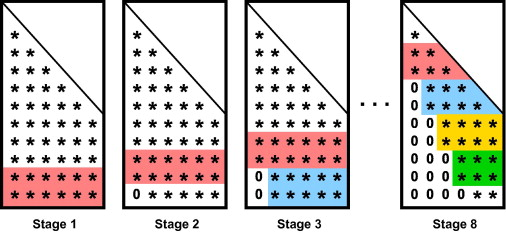
\includegraphics[width=0.8\linewidth]{Applying-Givens-rotations-in-parallel.png}
    \caption{Visualization of the MPI Givens algorithm.}
    \label{fig:mpi_givens}
\end{figure}



\subsubsection{General Observations and Recommendations}

The MPI approach theoretically aims for a speedup of \( \frac{n}{2} \), although the actual performance is hardly influenced by the data movement. This should be improved by avoiding the movement of the whole matrix between every processor.

Below in figure~\ref{fig:speedup_comparison} are the presented results:

\begin{figure}[h]
    \centering
    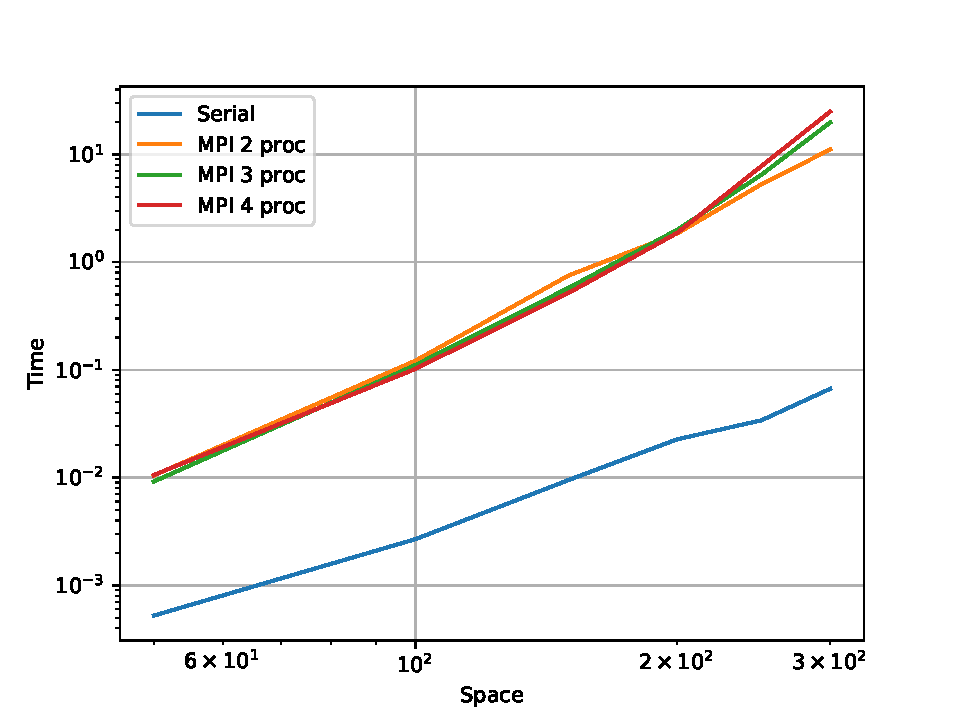
\includegraphics[width=0.5\linewidth]{mpi.pdf}
    \caption{Speedup comparison between MPI and OpenMP implementations.}
    \label{fig:speedup_comparison}
\end{figure}

These results don't highlight any significant improvement in performance, particularly for larger matrix sizes. The MPI approach showcases a bottleneck with respect to data movement, which we weren't able to fix in time.






\subsection{Overview of Householder Algorithm}

The Householder algorithm is another numerical technique used for QR factorization, a process that decomposes a matrix into the product of an orthogonal matrix \(Q\) and an upper triangular matrix \(R\). Similar to the Givens algorithm, the Householder transformation is employed to introduce zero elements below the diagonal of the matrix.

We provided two implementations, since our first implementation showd some low performances for bigger matrix. For this reason, we will discuss only the most performant implementation. All the results are showe at figure~\ref{fig:speedup_comparison_qr} .
The implementation provided, the Householder algorithm is applied to a given matrix $A$ to obtain its QR factorization, where $Q$ is an orthogonal matrix and $R$ is an upper triangular matrix.

\begin{algorithm}
\caption{QR Decomposition with Householder Transformation}
\begin{algorithmic}[1]
\Function{lec18hqr1}{$A$}
    \State $[m, n] \gets \text{size}(A)$
    \State $Q \gets \text{eye}(m)$ \Comment{Initialize orthogonal transform}
    \State $R \gets A$ \Comment{Initialize transformed matrix}
    
    \For{$j \gets 1$ \textbf{to} $n$}
        \State \Comment{Find $H = I - \tau \cdot w \cdot w'$ to put zeros below $R(j, j)$}
        \State $normx \gets \text{norm}(R(j{:}, j))$
        \State $s \gets -\text{sign}(R(j, j))$
        \State $u1 \gets R(j, j) - s \cdot normx$
        \State $w \gets R(j{:}, j) / u1$
        \State $w(1) \gets 1$
        \State $\tau \gets -s \cdot u1 / normx$
        
        \State \Comment{Update $R$: $R \gets HR$, $Q$: $Q \gets QH$}
        \State $R(j{:}, :) \gets R(j{:}, :) - (\tau \cdot w) \cdot (w^T \cdot R(j{:}, :))$
        \State $Q(:, j{:}) \gets Q(:, j{:}) - (Q(:, j{:}) \cdot w) \cdot (\tau \cdot w^T)$
    \EndFor
    
    \State \textbf{return} $(Q, R)$
\EndFunction
\end{algorithmic}
\end{algorithm}

It should be noticed that such implementation avoids explicitly to construct the Givens rotation matrix and directly computes the changes to matrices $Q$ and $R$ during each iteration. This approach can be computationally efficient, especially for large matrices.

\subsubsection{Parallelization}
The Householder algorithm was parallelized using OpenMP directives to improve its computational efficiency. The parallelization was strategically applied to different parts of the algorithm to exploit concurrent processing capabilities.

In the section responsible for calculating the norm (normx), OpenMP parallelization was employed. This involved distributing the workload across multiple threads, each contributing to the summation of squared elements in the specified range of the matrix R. A reduction clause ensured the correct accumulation of the norm, and subsequent computations were encapsulated within a single section.

The initialization of the vector w was parallelized, with individual threads assigned to compute distinct portions of the vector. Outside the loop, the value w(j, 0) was set independently within a single section.

The computation of temporary vectors and matrices, such as \texttt{tmp\_R}, \texttt{R}, \texttt{tmp\_Q}, and \texttt{Q}, was parallelized using OpenMP directives. For instance, the calculation of the temporary vector \texttt{tmp\_R} was distributed among threads. Nested loops involved in updating matrices \texttt{R} and \texttt{Q} were parallelized using the \texttt{collapse(2)} clause, optimizing thread utilization.

The final section involved resetting temporary vectors (\texttt{tmp\_R} and \texttt{tmp\_Q}) and the variable \texttt{normx}. This operation was enclosed in a single section to ensure that the reset was performed by a single thread, avoiding potential race conditions.


The parallelization strategy aimed to maximize concurrency, efficiently utilizing available computational resources, and ultimately reducing the overall execution time of the Householder algorithm. Each pragma-annotated section denoted a specific part of the algorithm where parallel execution was strategically applied.


\subsection{Computational Considerations}
One can assert that, in general, for dense matrices, it is advantageous to use the Householder algorithm for QR factorization. On the other hand, if the matrix to be factorized already has many zero diagonals below the main diagonal, then the Givens algorithm may be more convenient from a computational perspective. This is based on both the reduced computation time and the fewer number of operations performed. The choice between Householder and Givens algorithms is influenced by the matrix structure and the specific requirements of the computation. Householder transformations are preferred for their numerical stability and efficiency in handling dense matrices, while Givens rotations are advantageous when dealing with matrices exhibiting sparsity, particularly with many zero diagonals below the main diagonal. This is shown in the figure~\ref{fig:sparsity_test}.


\subsection{Results and Performance}
Both algorithms respond well to the increase in size, with givens being a bit more scalable. Householder tends to be a bit quicker serially, which is in line with the theory.
Speedup diagram looks to be valuable from sizes of around 150x150 due to the big overhead related to the creation of the threads.
Finally, sparsity plays a big role in the performance of these algorithms. In particular, we can see in figure~\ref{fig:sparsity_test} how the performance of the Givens rotation algorithm increases proportionally to the zeros of the subdiagonal part of the input matrix. For dense matrix, depending on the input matrix, the two algorithm looked comparable as shown in figure~\ref{fig:timeQR}.


    \begin{figure}[htbp]
    \begin{minipage}{0.3\textwidth}
        \centering
        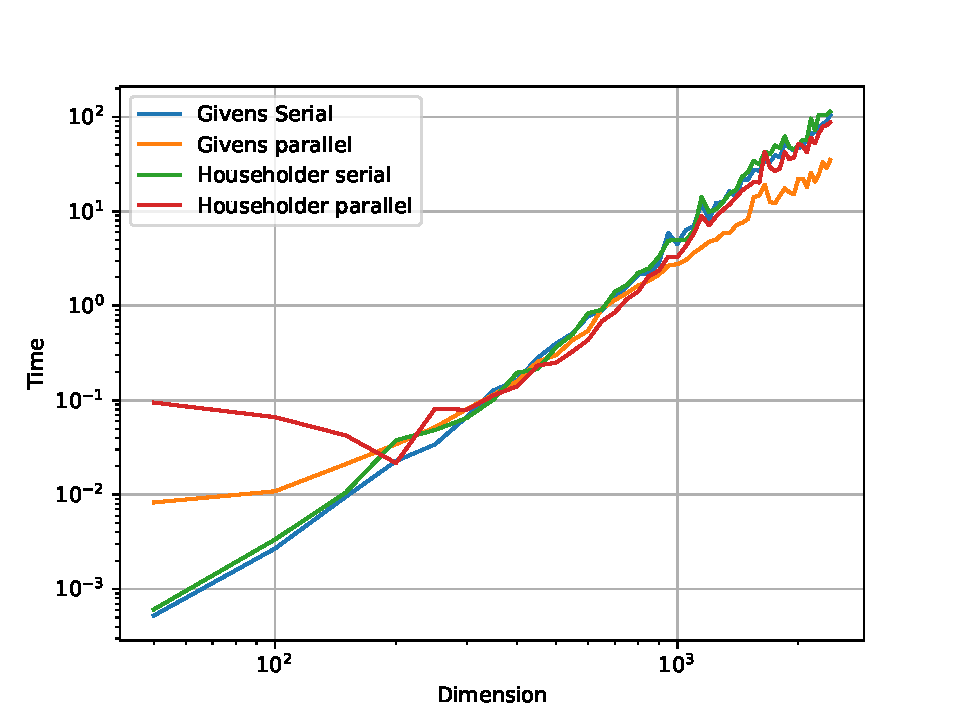
\includegraphics[width=\textwidth]{timeQR.pdf}
        \caption{Time Duration with respect to size}
        \label{fig:timeQR}
    \end{minipage}%
    \hfill
    \begin{minipage}{0.3\textwidth}
        \centering
        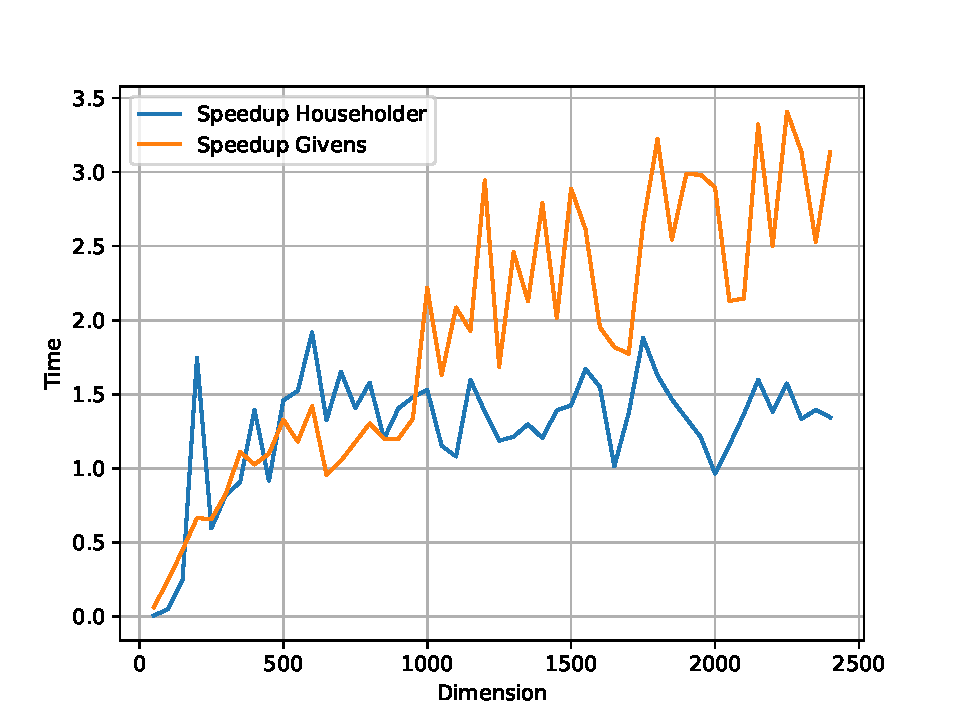
\includegraphics[width=\textwidth]{SpeedUpQR.pdf}
        \caption{Speedup with respect to size}
        \label{fig:spQR}
    \end{minipage}%
    \hfill
    \begin{minipage}{0.3\textwidth}
        \centering
        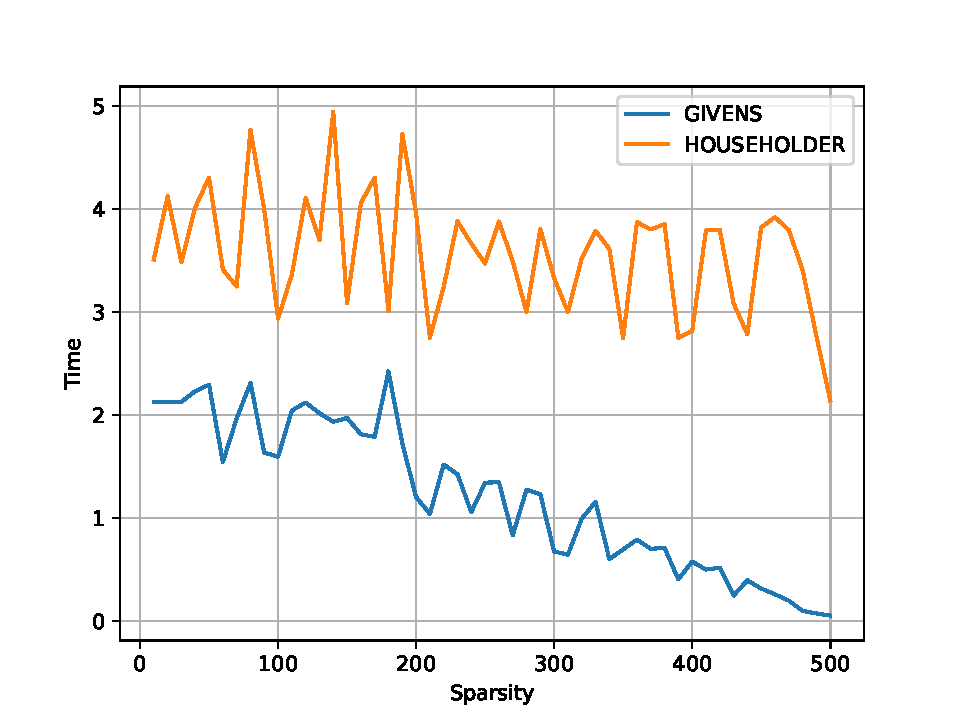
\includegraphics[width=\textwidth]{sparsity.pdf}
        \caption{Time duration with mpi}
        \label{fig:sparsity_test}
    \end{minipage}
\end{figure}








    
\newpage

\section{MATRIX IMPLEMENTATION}

In order to perform the operations described above, a custom \texttt{Matrix} class has been developed.

The class is generic with respect to the type saved in the matrix (preferably a floating point), and it has another template parameter which is the ordering, either row-major or col-major.

The decision of the ordering is done at compile time, so the implementation has the choice to select the best implementation with no overhead at runtime.

The \texttt{FullMatrix} class has been developed in parallel with all the algorithms, so the first implementation contained the matrix classes provided by the Eigen library.

In order to avoid the rewriting of the code, all the methods provided by the \texttt{FullMatrix} class have been created to emulate most of the Eigen functionalities. Indeed, if a particular method was utilized from the \texttt{Eigen::MatrixXd} class, it would appear a few days later also in the \texttt{FullMatrix} class.

\textbf{Note:} most of the functionalities are mirrored, but some could not be exactly replicated due to the inherently different structure (and surely, more complex) of the Eigen library. So in some parts of the code, there is a preprocessor directive:

\begin{verbatim}
#ifdef EIGEN

// Eigen::MatrixXd

#else 

// FullMatrix

#endif
\end{verbatim}

\textbf{Note:} Eigen uses another class for the definition of a vector, indeed \texttt{Eigen::VectorXd}. But the \texttt{FullMatrix} class can be also used as a vector; indeed, in the file \texttt{utils.hpp} there is:

\begin{verbatim}
using Vector = FullMatrix<Real, ORDERING::ROWMAJOR> // Real is a double
\end{verbatim}

\textbf{Remember:} there is an overload of the constructor of \texttt{FullMatrix} defined as

\begin{verbatim}
FullMatrix(const size_t n): FullMatrix(n,1) {}
\end{verbatim}

which creates a column vector.

So the accessing can be performed both in a matrix way, using the \texttt{operator()}, and in a vector way, using the \texttt{operator[]}.


\subsection{TRANSPOSITION}

The first implementation, when calling the method \texttt{transpose()}, would return a copy of the matrix but with the entries rearranged in order to satisfy the transposition.

This, of course, is not a good implementation since we are creating another matrix with all the information already present in the original one. With just one change of perspective, we can achieve much better performances.

Indeed, a class \texttt{FullMatrixAdjoint} has been developed that contains a reference to a \texttt{FullMatrix} object. When calling the access operators on a \texttt{FullMatrixAdjoint} object, it returns the elements in the matrix but from a transposed point of view (everything is mirrored with respect to the original object).

Note that this class is not a child of a \texttt{FullMatrix}, but a wrapper. This decision was made because conceptually a parent should not call methods that return its child, which happens in the \texttt{transpose()} method. But, of course, this decision has its disadvantages, since each method has to be re-declared from scratch (here in the class only the necessary methods have been developed).

The more correct solution would be similar to the Eigen implementation, each matrix class should derive from a superclass (called \texttt{MatrixBase} in Eigen) where most of the methods are defined.

Small note: there is some code repetition in the matrix class, since the matrix multiplication needs to be specified for matrix-transposed and the reverse, and for transposed-expression and reverse.

A better solution is to perform a partial specialization of the method with a concept (defined for matrix and its transposed), but there was a problem since I could not create a concept for the \texttt{FullMatrixTransposed} class. The type should be something along the lines of \texttt{FullMatrix<Real, ORDERING>::FullMatrixAdjoint}, but no matter the template I created, the compiler continued to give an error for the type declaration of the class.

\subsection{MULTIPLICATION}

The matrix can perform most of the classical component-wise operations (see section on lazy evaluation) and row-column operations.

Then the most expensive operation with matrices is the matrix-matrix multiplication, and here we briefly discuss some results.

The operation has been constructed following the article: \url{https://siboehm.com/articles/22/Fast-MMM-on-CPU}. Almost everything described has been implemented, except for the tiling of the operation.

The implementation is different for row-major and col-major matrices, and for both cases, it tries to exploit completely cache coherency and SIMD operations.

The results below show the performance of the matrix-matrix multiplication for increasing sizes of the matrices, both without compiler optimization and with the flags \texttt{"-O3 -march=native"} activated.

\begin{figure}
    \centering

    \subfloat[Photo of sumlong\_nolazy.png]{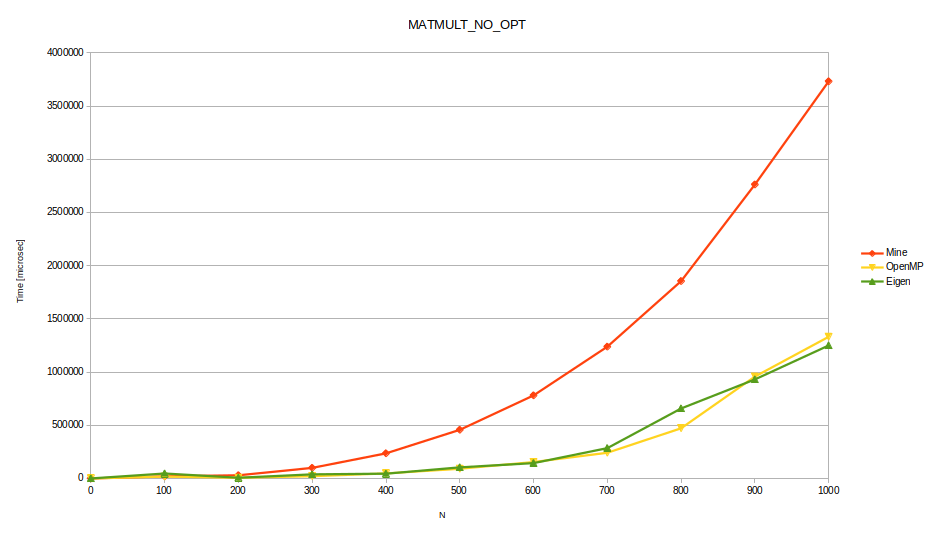
\includegraphics[width=0.5\textwidth]{matmult_noopt.png}\label{fig:sub1}}
    \hfill
    \subfloat[Photo of sumlong\_lazy.png]{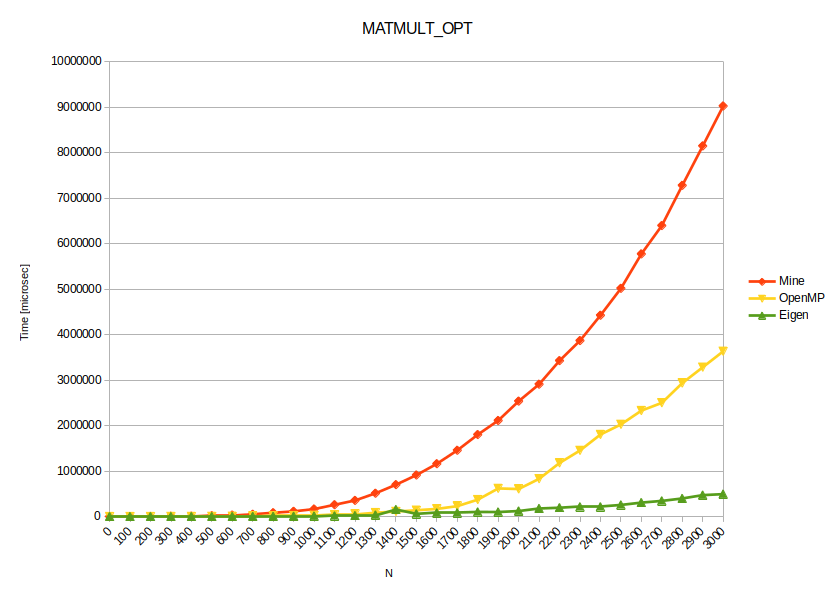
\includegraphics[width=0.5\textwidth]{matmult_opt.png}}\label{fig:sub4}

    \end{figure}

Here we can notice two main properties:

\begin{itemize}
    \item the optimizer does a lot of work (for \(N=1000\) we get approximately 70x speedup).
    \item up until approximately \(N=1600\) the OpenMP implementation keeps the pace with Eigen (which has also OpenMP beneath), but after that, there is a huge loss in performance, since the implementation does not perform tiling and the matrices are too big to fit in a single page of the cache.
\end{itemize}

\subsection{LAZY EVALUATION}

The matrix can also perform component-wise operations in a lazy way, by setting the compilation flag \texttt{"-DLAZY"}.

The pattern used is the CRTP (curiously recursive template pattern) of the expression templates, described extensively [here](https://link.springer.com/article/10.1007/s00791-009-0128-2).

This pattern helps construct an expression class at compile time that contains the expression tree evaluated by the compiler. Indeed, each class derives from a superclass \texttt{Expr<T>} recursively in the following way:

\begin{verbatim}
public class C : Expr<C> {…}
\end{verbatim}

There was also the possibility to construct lazily the row-column product, but this implementation was held back mainly by two major problems:

\begin{itemize}
    \item the optimization for cache-friendly accesses would require the multiplication operator (defined as a functor) to know about the ordering of the matrix at compile time and to reorder the operations accordingly.
    \item there is a major problem when performing an operation such as:

    \begin{verbatim}
    FullMatrix a;

    a = a * a; // Assuming that a is squared
    \end{verbatim}

    If the operation is performed in a lazy way, the result will, of course, not be correct starting from the second term computed in the matrix.

    An alternative solution then would require understanding at compile time if a matrix is present both in the lhs and the rhs of the operation, but the solution is not trivial and requires traversing the expression tree recursively at compile time.

    A simpler solution could also be to create a temporary each time the multiplication operator between matrices (or expressions of matrices) is called, but this is exactly what is done without expression templates. This would also not impact the performance much since creating a matrix is less costly than performing a multiplication.

    So in the end this operation was kept without lazy evaluation.
\end{itemize}

\textbf{Note:} the same problem emerges when doing an operation such that

\begin{verbatim}
a = a + (or -) a.transpose();
\end{verbatim}

Which returns the symmetric (or skew-symmetric) part of a matrix, but since it is not required from the application it was not addressed.

The tests in order to understand the improvements were performed on 5 different operations, both in a lazy and non-lazy way, all with the optimization flags enabled:

\begin{itemize}
    \item \texttt{c = a + b; // SUM\_SHORT}
    \item \texttt{c = a + b + a + b + a + b + a + b + a + b; // SUM\_LONG}
    \item \texttt{c = a * 2.; // PROD\_SHORT}
    \item \texttt{c = a * 2. * 2. * 2. * 2. * 2. * 2. * 2. * 2. * 2.; // PROD\_LONG}
    \item \texttt{c = a * (a + b * 2.) * a.transpose(); // MIXED}
\end{itemize}

\begin{figure}
    \centering

    \subfloat[Photo of sumlong\_nolazy.png]{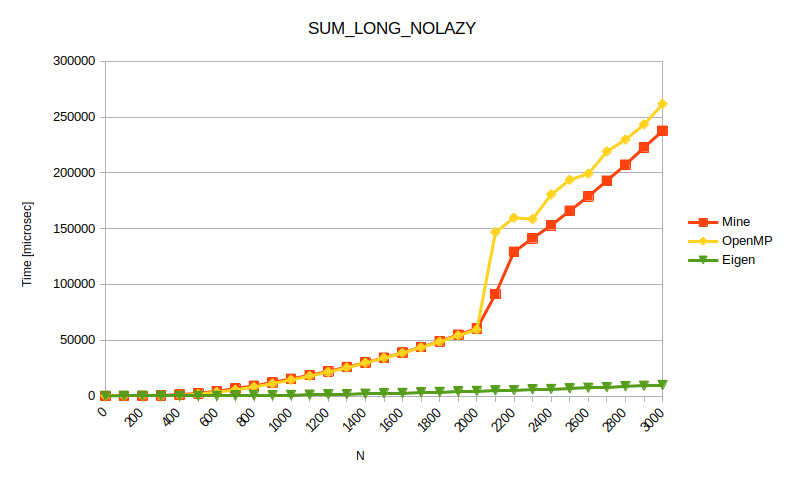
\includegraphics[width=0.5\textwidth]{sumlong_nolazy.png}\label{fig:sub1}}
    \hfill
    \subfloat[Photo of sumlong\_lazy.png]{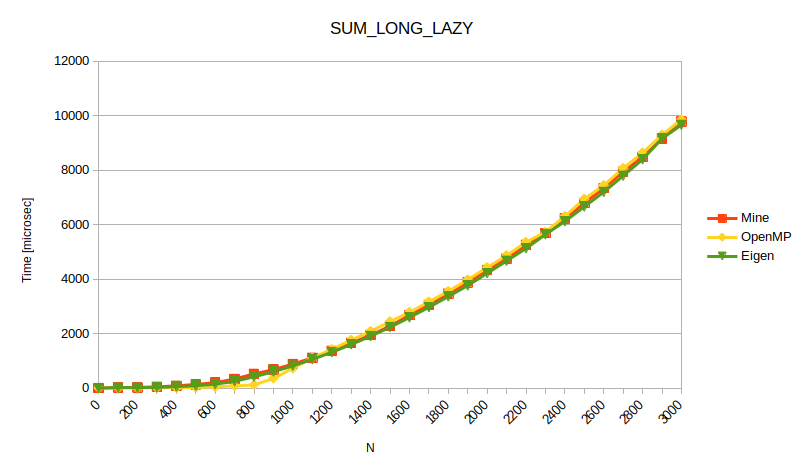
\includegraphics[width=0.5\textwidth]{sumlong_lazy.png}}\label{fig:sub4}
    

    \vspace{1em} % Spacing between the rows of images

    \subfloat[Photo of sumshort\_nolazy.png]{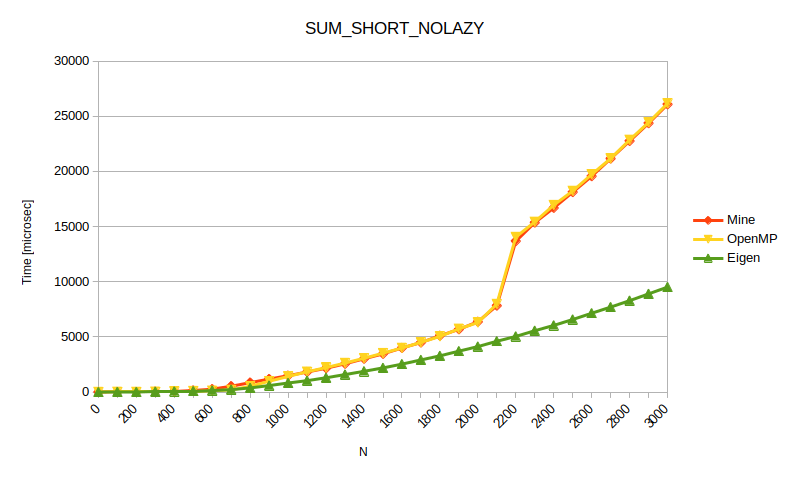
\includegraphics[width=0.5\textwidth]{sumshort_nolazy.png}\label{fig:sub3}}
    \hfill
    \subfloat[Photo of sumshort\_lazy.png]{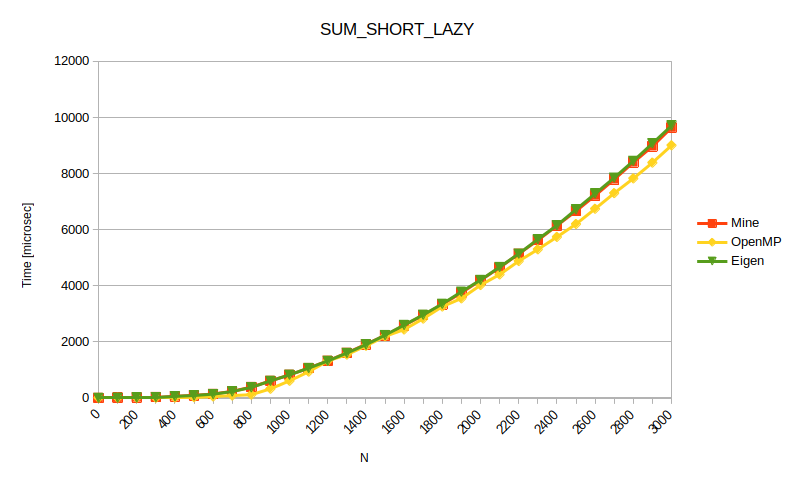
\includegraphics[width=0.5\textwidth]{sumshort_lazy.png}\label{fig:sub2}}
    \vspace{1em} % Spacing between the rows of images

    \subfloat[Photo of prodshort_lazy.png]{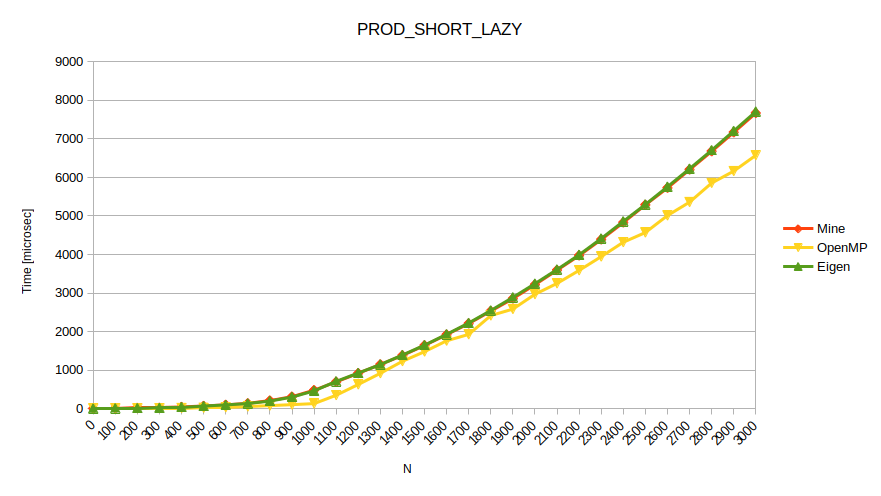
\includegraphics[width=0.5\textwidth]{prodshort_lazy.png}\label{fig:sub3}}
    \hfill
    \subfloat[Photo of mixed_nolazy.png]{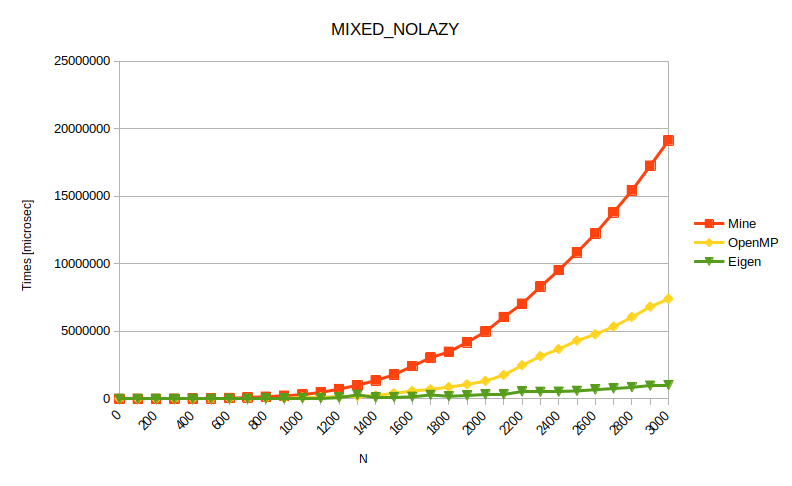
\includegraphics[width=0.5\textwidth]{mixed_nolazy.png}\label{fig:sub2}}
    \vspace{1em} % Spacing between the rows of images

    \subfloat[Photo of prodshort_lazy.png]{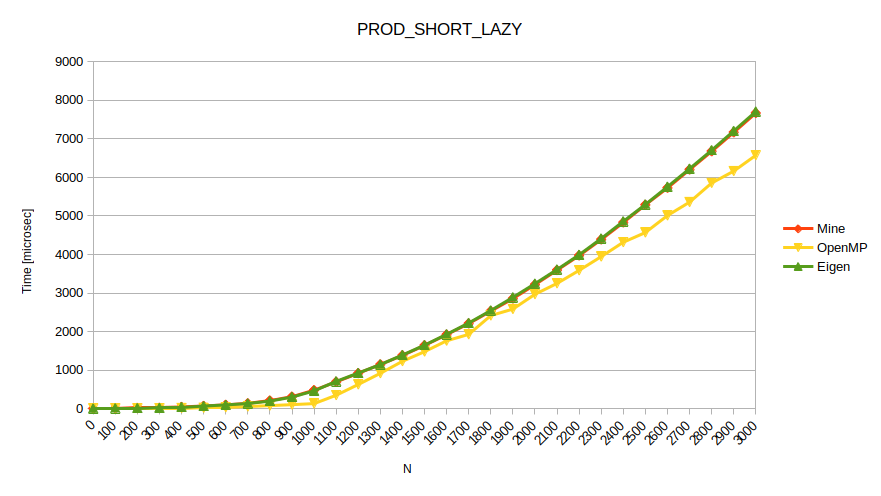
\includegraphics[width=0.5\textwidth]{prodshort_lazy.png}\label{fig:sub3}}
    \hfill
    \subfloat[Photo of mixed_lazy.png]{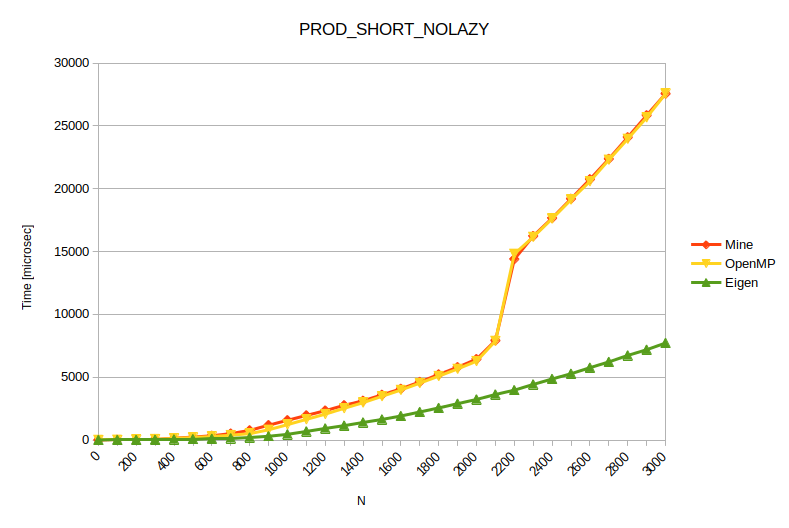
\includegraphics[width=0.5\textwidth]{prodshort_nolazy.png}\label{fig:sub2}}

    \caption{Impact of lazy evaluation on matrix sum}
    \label{fig:lazy_nolazy_prod}
\end{figure}

Here we can see that using lazy evaluation on the sum of matrices has a huge impact since for the long operation the speedup reaches 25x.

Now since this operation is not very realistic, we can see that only with a small operation we get an approximate 2.5x speedup, and since is just 1 against the 9 sums of before, the results are expected (we create 9 temporaries and do a last assignment -> 10 operations in total).

Also for the product of multiple scalars, we get a similar speedup, this time is actually higher since we have to do fewer accesses to the memory because we work only with one matrix.

Interestingly, we can see that for the lazy product, an OpenMP implementation gives some performance increase, not much but it is still approximately a 1.1x speedup.

For a mixed operation, we can see that the graph very much resembles the matrix-matrix multiplication, just with a lot more time since now we perform 3 multiplications.

So if we would like an improvement from the timing perspective, we would need to increase much more the size of the lazy expression, but it is not realistic since it is not in any of the algorithms implemented. But at least there is an improvement in memory usage, since fewer temporaries are created.

\subsection{BENCHMARKS}

The specifics of my computer are the following:

\begin{figure}[htbp]
    \centering
    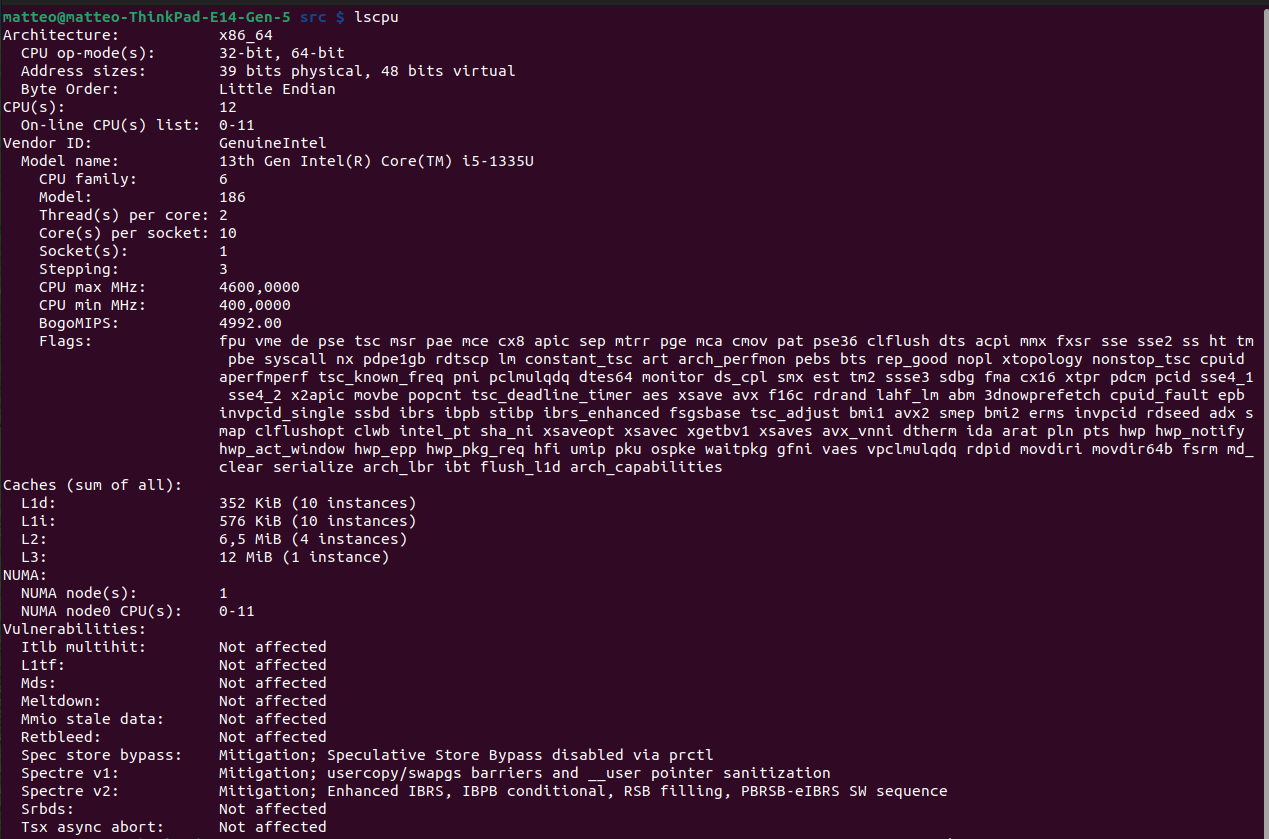
\includegraphics[width=0.4\textwidth]{my_specs.png}
    \caption{Photo of my\_specs.png}
\end{figure}

All the tests are performed using a benchmark that executes the operations a bunch of times for different sizes of the matrices.

Then the best-performing time (the fastest) is kept after all the tests have been done and stored in a CSV file.

The formula for how many iterations have to be performed is the following exponential:

\[\text{times} = \text{floor}(2. + (\text{end} – 2.) \times \exp\left((\text{tau}/\text{end})\times(\text{start}-\text{i})))

where \(i\) is the current dimension of the matrix, \(\text{{start}}\) is the initial dimension, \(\text{{end}}\) is the final dimension, and \(\tau\) is a constant decided differently for each operation.

\textbf{Small note:} In the code, there is also a linear interpolator and a cubic interpolator, but the cubic does not work well, and the linear does not reflect well the difference in time/size with the matrix multiplication (since it grows as a cubic function).


\end{document}
